\chapter{Reproducción asexual y clonación en las plantas}\label{ch:b2:asexual-reproduction}

En un valle de Utah se alza un bosque de cuarenta y siete mil troncos de
álamo temblón que es una sola planta: todos los troncos han crecido del
mismo sistema de raíces, todas las células llevan el mismo genoma, y el
individuo tiene unos catorce mil años y pesa seis mil toneladas. Todas
las fresas de una bandeja de supermercado de una misma variedad son
fragmentos de una sola planta multiplicada por estolones; todos los
plátanos Cavendish de la Tierra son esquejes de esquejes de una sola
planta. Las plantas, a diferencia de la mayoría de los animales, pueden
formar nuevos individuos sin sexo --- a partir de un tallo, una raíz,
una hoja, una sola célula en un matraz. Este capítulo examina cómo lo
hacen, cómo lo aprovechan los cultivadores y qué le cuesta a un linaje
renunciar a la \omterm{def:b2:meiosis-heredity:meiosis}{meiosis} y a la fecundación: la cuestión de por qué existe
el sexo.

\section{Multiplicación vegetativa}

\begin{definition}[Clon, geneto, rameto]\label{def:b2:asexual-reproduction:clone}
\index{clon}\index{geneto}\index{rameto}\index{multiplicación vegetativa}
La \emph{reproducción asexual} produce nuevos individuos a partir de un
solo progenitor solo por mitosis, sin \omterm{def:b2:meiosis-heredity:meiosis}{meiosis} ni fecundación: los
descendientes forman un \emph{clon}, genéticamente idéntico al
progenitor y entre sí, salvo por las \omterm{def:b2:genome-diversification:mutation}{mutaciones} somáticas que se
acumulan. En las plantas la forma habitual es la \emph{multiplicación
vegetativa}, en la que una parte del cuerpo --- tallo, raíz, hoja ---
echa raíces y se convierte en una planta separada. Un \emph{geneto} es el
individuo genético, todo lo que ha crecido a partir de un cigoto; un
\emph{rameto} es una unidad fisiológicamente separada de él. Un bancal de
fresas puede contener mil rametos de un solo geneto; el bosque de álamos
es un solo geneto. La multiplicación vegetativa es posible porque las
células vegetales conservan la capacidad de dividirse y de formar
cualquier órgano --- son \emph{totipotentes} --- y porque las plantas
crecen a partir de meristemos que pueden reactivarse casi en cualquier
lugar.
\end{definition}

\begin{proposition}[Los órganos de la multiplicación vegetativa]\label{prop:b2:asexual-reproduction:organs}
\index{estolón}\index{rizoma}\index{tubérculo}\index{bulbo}
Las plantas han desarrollado el mismo recurso a partir de todos sus
órganos. A partir de tallos: \emph{estolones} o \emph{guías}, tallos
horizontales a ras de suelo que enraízan en sus nudos (fresa, botón de oro rastrero);
\emph{rizomas}, tallos subterráneos horizontales que se ramifican y se
fragmentan (grama, lirio, jengibre, \omterm{def:b2:plant-life-cycles:fern}{helecho} común); \emph{tubérculos},
extremos hinchados de rizomas que almacenan almidón y llevan yemas, los
``ojos'' (patata); \emph{cormos}, bases de tallo verticales hinchadas
(azafrán); \emph{bulbilos}, pequeños bulbos formados en las axilas de las
hojas o en la inflorescencia (ajo, algunas cebollas). A partir de hojas:
\emph{bulbos}, yemas envueltas en hojas carnosas de reserva que se
dividen en bulbos hijos (cebolla, tulipán); plántulas a lo largo del
borde de la hoja, provistas de raíces, que se desprenden
(\emph{Kalanchoe}). A partir de raíces: \emph{retoños}, brotes que surgen
de raíces horizontales (álamo temblón, endrino, frambueso). Por
\emph{fragmentación}: un trozo de rama de sauce que la corriente arrastra
y que echa raíces, una fronda de lenteja de agua que se divide. En todos
los casos un órgano de reserva o un meristemo se desplaza una corta
distancia, y la planta hija empieza su vida con una provisión de
alimento que ninguna \omterm{def:b2:angiosperm-reproduction:seed}{semilla} puede igualar.
\end{proposition}

\begin{omfigure}
\begin{tikzpicture}[every node/.style={font=\scriptsize}]
  % runner
  \begin{scope}
    \draw[thick] (0,0) -- (3.6,0);
    \foreach \x in {0,1.8} { \draw[thick, omExo!70!black, fill=omExo!30] (\x,0) .. controls (\x-0.3,0.6) and (\x+0.3,0.6) .. (\x,0); \foreach \a in {60,90,120} \draw[thick, omExo!70!black] (\x,0) -- ++(\a:0.7); \draw[gray] (\x,0) -- ++(-100:0.4) (\x,0) -- ++(-70:0.4); }
    \draw[thick, omThm] (0.2,0.15) .. controls (0.9,0.55) and (1.2,0.55) .. (1.8,0.1);
    \draw[thick, omThm] (2.0,0.15) .. controls (2.7,0.55) and (3.0,0.55) .. (3.5,0.1);
    \draw[thick, omExo!70!black] (3.5,0.1) -- ++(80:0.4); \draw[gray] (3.5,0.1) -- ++(-80:0.3);
    \node[below, align=center] at (1.8,-0.55) {estolón (fresa):\\un tallo horizontal enraíza en sus nudos};
  \end{scope}
  % rhizome and tuber
  \begin{scope}[xshift=5.2cm]
    \draw[gray, dashed] (-0.2,0) -- (3.8,0);
    \draw[very thick, omProp!80!black] (0,-0.5) -- (3.4,-0.5);
    \foreach \x in {0.6,2.0} \draw[thick, omExo!70!black] (\x,-0.5) -- (\x,0.7) (\x,0.3) -- ++(40:0.4) (\x,0.3) -- ++(140:0.4);
    \draw[thick, omProp!80!black, fill=omProp!40] (3.4,-0.5) ellipse (0.45 and 0.3);
    \foreach \p in {(3.2,-0.3),(3.6,-0.35),(3.7,-0.6)} \fill[omThm] \p circle (0.04);
    \foreach \x in {0.3,1.3,2.5} \draw[gray] (\x,-0.5) -- (\x,-0.9);
    \node[below, align=center] at (1.8,-1.05) {rizoma y tubérculo (patata):\\tallos subterráneos,\\yemas (ojos) en el tubérculo};
  \end{scope}
  % bulb
  \begin{scope}[xshift=12.2cm]
    \draw[thick, fill=omExo!15] (0,-0.9) .. controls (-0.9,-0.6) and (-0.9,0.9) .. (0,1.0) .. controls (0.9,0.9) and (0.9,-0.6) .. (0,-0.9);
    \foreach \r in {0.55,0.35} \draw[thick] (0,-0.75) .. controls (-\r,-0.5) and (-\r,0.6) .. (0,0.8) .. controls (\r,0.6) and (\r,-0.5) .. (0,-0.75);
    \fill[omExo!60!black] (-0.1,-0.75) rectangle (0.1,0.3);
    \draw[thick, omThm, fill=omThm!30] (0.35,-0.5) ellipse (0.15 and 0.3);
    \foreach \x in {-0.3,0,0.3} \draw[gray] (\x,-0.9) -- (\x,-1.25);
    \node[below, align=center] at (0,-1.3) {bulbo (cebolla):\\hojas carnosas,\\un bulbo hijo (rojo)};
  \end{scope}
\end{tikzpicture}

{\small Tres órganos de \omterm{def:b2:asexual-reproduction:clone}{multiplicación vegetativa}: estolones que enraízan
en sus nudos, un tallo subterráneo que se hincha en un tubérculo y un
bulbo que forma un bulbo hijo. En todos los casos una yema viaja con su
alimento.}
\end{omfigure}

\begin{omfigure}
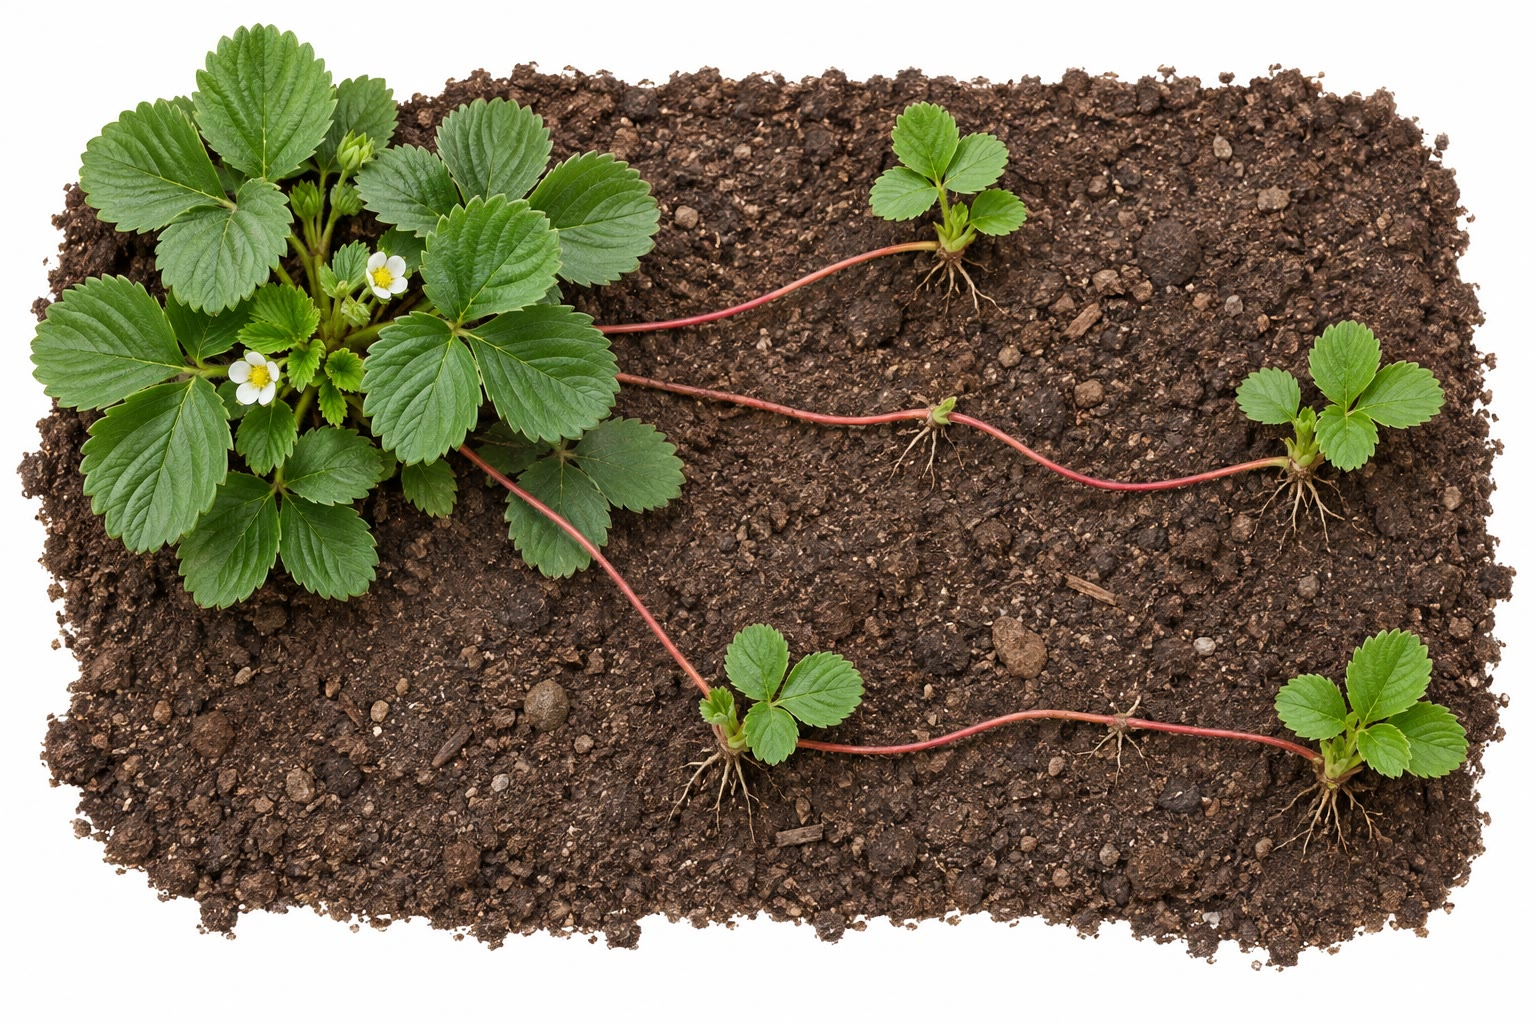
\includegraphics[width=0.46\linewidth]{images/book4/ai/b4-07-strawberry-runners.jpg}\hspace{0.03\linewidth}
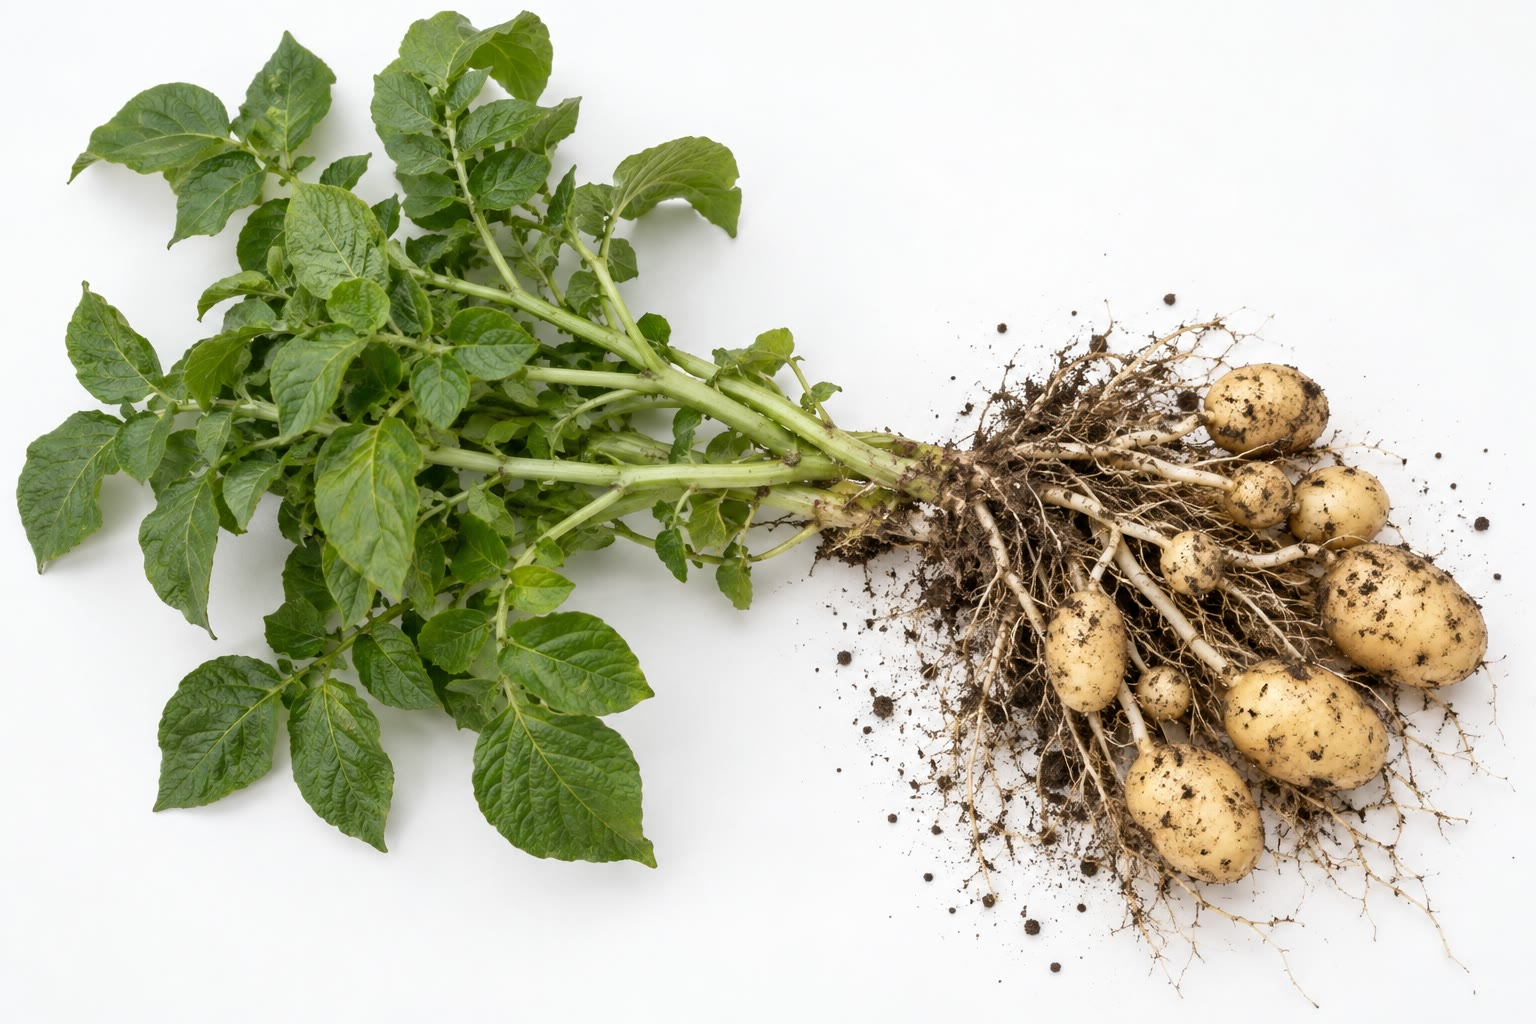
\includegraphics[width=0.46\linewidth]{images/book4/ai/b4-07-potato-tubers.jpg}

{\small Izquierda: una planta de fresa y las plantas hijas que enraízan a
lo largo de sus estolones. Derecha: una planta de patata sacada de la
tierra, con los tubérculos colgando de los estolones --- cada tubérculo
es un trozo de tallo que dará una planta genéticamente idéntica a esta.}
\end{omfigure}

\begin{theorem}[La geometría de un clon que se extiende]\label{thm:b2:asexual-reproduction:spread}
\index{crecimiento clonal}
Un \omterm{def:b2:asexual-reproduction:clone}{geneto} en el que cada \omterm{def:b2:asexual-reproduction:clone}{rameto} produce cada año $m$ hijos enraizados,
todos supervivientes, crece en número como $N(t) = N_0 (1 + m)^t$ ---
crecimiento exponencial sin ningún sexo --- hasta que los \omterm{def:b2:asexual-reproduction:clone}{rametos} llenan
el espacio a su densidad de carga $d$ (\omterm{def:b2:asexual-reproduction:clone}{rametos} por unidad de
superficie), tras lo cual el \omterm{def:b2:asexual-reproduction:clone}{clon} avanza como un frente. Un \omterm{def:b2:asexual-reproduction:clone}{clon} que
extiende sus estolones en línea recta a velocidad $v$ tiene, al cabo de
$t$ años, un radio $vt$, y el número de \omterm{def:b2:asexual-reproduction:clone}{rametos} crece como
$\pi d (vt)^2$: de forma cuadrática, no exponencial. Una planta de fresa
que emite estolones de \qty{0.5}{m} al año tiene un radio de \qty{5}{m}
al cabo de diez años; el \omterm{def:b2:asexual-reproduction:clone}{clon} de álamos del párrafo inicial,
de \qty{43}{ha}, tiene un radio de unos \qty{370}{m} y, con un avance
neto de unos pocos centímetros al año, una edad del orden de $10^{4}$
años --- coherente con la edad estimada a partir del retroceso de los
glaciares.
\end{theorem}
\begin{proof}
Cada año cada \omterm{def:b2:asexual-reproduction:clone}{rameto} es sustituido por sí mismo más $m$ hijos, un factor
$1 + m$; $t$ años dan $(1 + m)^t$. Una vez lleno el interior, solo los
\omterm{def:b2:asexual-reproduction:clone}{rametos} del borde encuentran espacio, y el borde avanza a la velocidad
de los estolones $v$; la superficie es $\pi(vt)^2$ y el número de \omterm{def:b2:asexual-reproduction:clone}{rametos}
es la superficie por la densidad.
\end{proof}

\begin{example}[Los organismos más antiguos]\label{ex:b2:asexual-reproduction:oldest}
El \omterm{def:b2:asexual-reproduction:clone}{clon} de álamo temblón Pando (Utah) cubre \qty{43}{ha} con unos
\num{47000} troncos que viven cada uno alrededor de un siglo y son
sustituidos por retoños de las mismas raíces; el \omterm{def:b2:asexual-reproduction:clone}{geneto} podría tener más
de diez mil años. Un \omterm{def:b2:asexual-reproduction:clone}{clon} de la fanerógama marina \emph{Posidonia} del
Mediterráneo se extiende \qty{15}{km} y podría tener cien mil años; un
anillo de gobernadora del desierto de Mojave se ha datado en
\num{11700} años, con los tallos centrales muriendo a medida que el
anillo se expande. En todos los casos lo antiguo es el \omterm{def:b2:asexual-reproduction:clone}{geneto}; ninguna
célula suya tiene más de unas pocas décadas, y el genoma se ha copiado
miles de veces.
\end{example}

\section{Semillas sin sexo y animales sin padre}

\begin{definition}[Apomixis]\label{def:b2:asexual-reproduction:apomixis}
\index{apomixis}\index{partenogénesis}
La \emph{apomixis} es la producción de \omterm{def:b2:angiosperm-reproduction:seed}{semillas} sin fecundación: un
embrión se desarrolla a partir de una oosfera no reducida (la célula
madre de la \omterm{def:b2:plant-life-cycles:heterospory}{megaspora} se salta la \omterm{def:b2:meiosis-heredity:meiosis}{meiosis}) o directamente a partir de una
célula de la nucela, y la \omterm{def:b2:angiosperm-reproduction:seed}{semilla} lleva el \omterm{def:b2:meiosis-heredity:vocabulary}{genotipo} de la madre. Lo hacen
los dientes de león, las vellosillas, las zarzamoras, la poa de los
prados y muchos cítricos; la \omterm{def:b2:angiosperm-reproduction:seed}{semilla} de los cítricos contiene a menudo
varios embriones, uno sexual y los demás copias nucelares de la madre.
La apomixis conserva la \omterm{def:b2:angiosperm-reproduction:seed}{semilla} --- su dispersión, su \omterm{def:b2:angiosperm-reproduction:seed}{latencia} y su
cubierta --- y prescinde de la \omterm{def:b2:meiosis-heredity:meiosis}{meiosis}, de modo que un \omterm{def:b2:meiosis-heredity:vocabulary}{genotipo} bien
adaptado se difunde sin cambios; la mayoría de los apomícticos son
\omterm{def:b2:genome-diversification:polyploidy}{poliploides} de origen híbrido cuya \omterm{def:b2:meiosis-heredity:meiosis}{meiosis} fracasaría de todos modos. El
equivalente animal es la \emph{partenogénesis}, el desarrollo a partir de
un óvulo no fecundado: obligada en algunos lagartos y en los rotíferos
bdeloideos, que llevan decenas de millones de años sin machos; cíclica en
los pulgones y las pulgas de agua, que se multiplican por partenogénesis
todo el verano, con hembras que paren hijas vivas que ya llevan sus
propios embriones, y que pasan en otoño a una generación sexual que pone
huevos de invierno.
\end{definition}

\begin{omfigure}
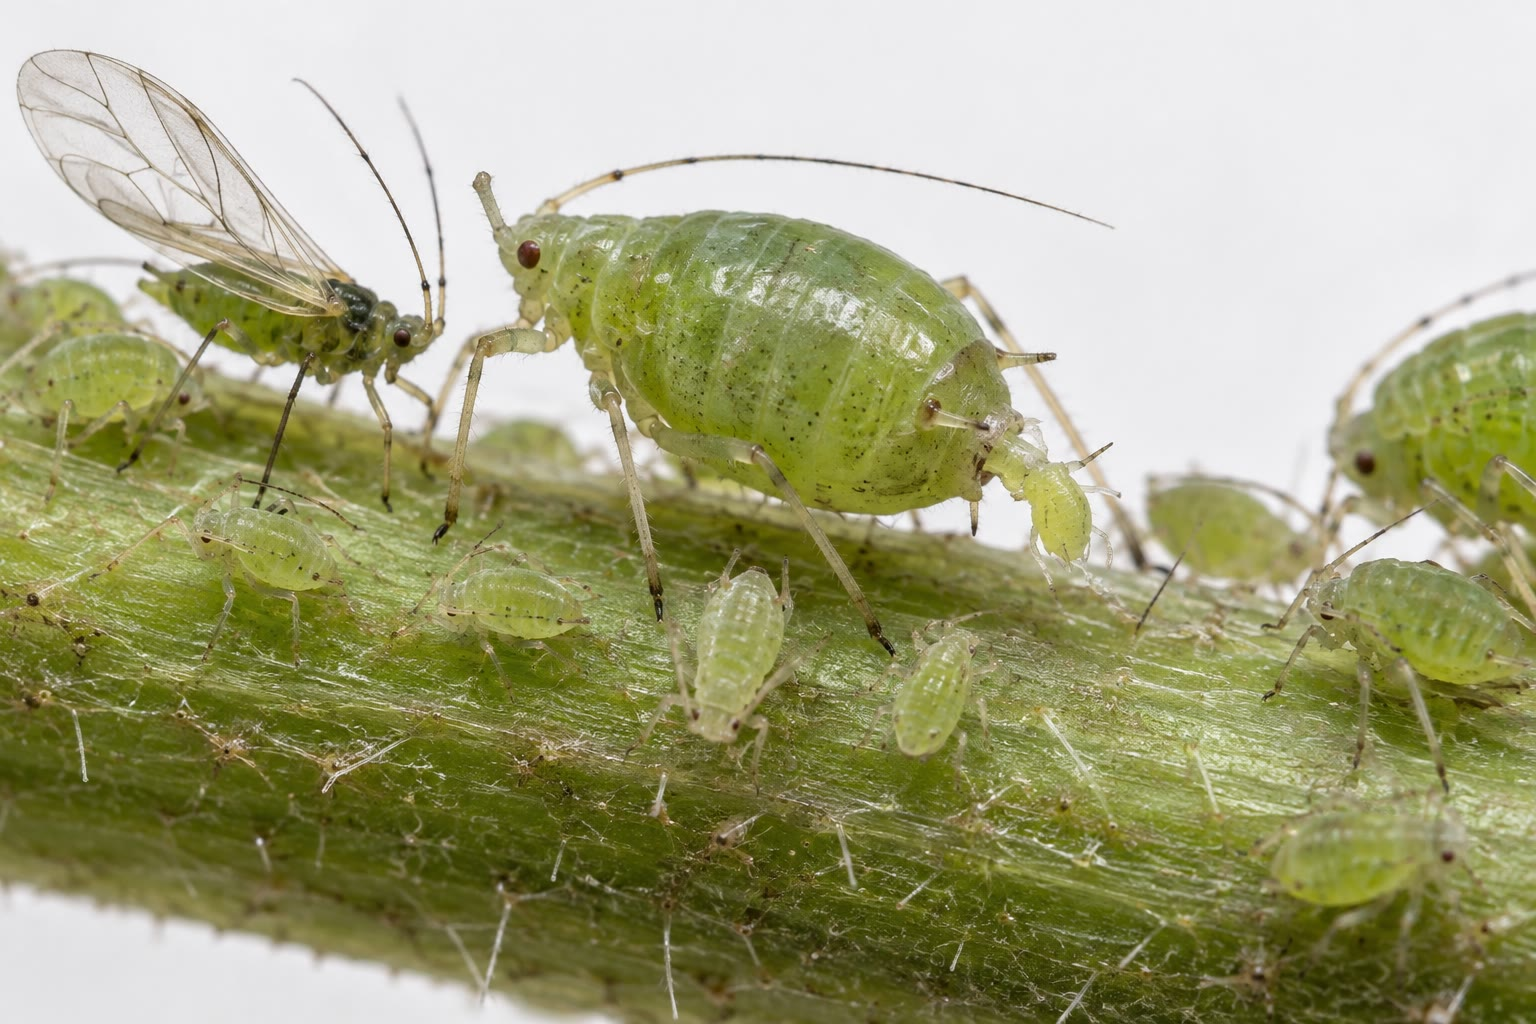
\includegraphics[width=0.55\linewidth]{images/book4/ai/b4-07-aphids.jpg}

{\small Pulgones sobre un tallo: una hembra partenogenética áptera que
pare una hija viva, ninfas de varias edades y una migrante alada --- el
crecimiento exponencial de un verano sin un solo macho.}
\end{omfigure}

\begin{example}[Un verano de pulgones]\label{ex:b2:asexual-reproduction:aphids}
Un pulgón partenogenético madura en unos ocho días y produce unas cinco
hijas al día durante dos semanas; las hijas nacen ya preñadas (los
embriones empiezan a desarrollarse dentro de los embriones de la madre).
Con un \omterm{def:b2:unicellular-diversity:division}{tiempo de generación} cercano a diez días y una tasa neta de
aumento de unos \num{50} por generación, una sola fundadora en abril
podría, sin freno, dejar $50^{12} \approx 2\times 10^{20}$ descendientes
en octubre --- una masa superior a la de la Tierra. Las mariquitas, las
crisopas, las avispas parasitoides, los hongos y la lluvia limitan su
número a unos pocos miles por planta, y la generación sexual de otoño
reinicia el \omterm{def:b2:asexual-reproduction:clone}{clon} en huevos recombinados antes del invierno.
\end{example}

\section{La clonación por el cultivador}

\begin{proposition}[Esquejes, acodos, injertos]\label{prop:b2:asexual-reproduction:horticulture}
\index{esqueje}\index{injerto}\index{portainjerto}
Un \emph{esqueje} es un trozo de tallo, raíz u hoja al que se induce a
enraizar: el extremo cortado forma un callo de células en división del
que surgen meristemos radiculares, con ayuda de auxina (la hormona de
enraizamiento) y humedad. El \emph{acodo} hace enraizar una rama
mientras sigue unida a la planta y la corta después. El \emph{injerto}
une un brote de una planta (la \emph{púa}) al tallo enraizado de otra (el \emph{portainjerto}): se ponen en
contacto los dos cámbiums, un callo tiende un puente sobre la herida, y
en pocas semanas un nuevo xilema y un nuevo floema lo atraviesan. El
injerto es una quimera --- las raíces conservan el genoma del
portainjerto; el brote que fructifica, el de la púa --- y solo funciona
entre plantas emparentadas (especies de un mismo género, a veces de una
misma familia), porque los tejidos deben reconocer las células del otro.
Todas las variedades de manzano, peral, cerezo, cítricos y vid se
propagan por injerto: una variedad con nombre es un solo \omterm{def:b2:asexual-reproduction:clone}{geneto},
mantenido vivo durante siglos mediante púas (las manzanas reinetas datan
del siglo XVI), y el portainjerto se elige según el suelo, la enfermedad
y el tamaño de árbol deseado --- los portainjertos enanizantes dan los
árboles pequeños de los huertos modernos.
\end{proposition}

\begin{proposition}[Micropropagación y totipotencia]\label{prop:b2:asexual-reproduction:tissueculture}
\index{micropropagación}\index{totipotencia}\index{callo}
Cualquier célula vegetal viva con núcleo puede, en principio, regenerar
una planta entera. En el \emph{cultivo de tejidos}, un fragmento de
tejido esterilizado (un \emph{explante}: un ápice caulinar, un disco de
hoja, una antera) se coloca en un medio de agar con azúcar, minerales,
vitaminas y hormonas. Con la auxina y la citoquinina en equilibrio, las
células se desdiferencian en un \emph{callo}, una masa de células no
especializadas en división; con más citoquinina que auxina, el callo
forma brotes; con más auxina que citoquinina, forma raíces; y en algunas
especies forma \emph{embriones somáticos} --- embriones completos sin
oosfera. Los brotes se cortan y se subcultivan cada pocas semanas, y se
multiplican por un factor de tres a diez cada vez, de modo que un
meristemo da un millón de plántulas en un año. Como los virus van por
detrás del ápice en crecimiento, un meristemo caulinar de menos de un
milímetro suele estar libre de virus incluso en una planta infectada: el
\emph{cultivo de meristemos} es la manera de sanear las existencias de
patata, fresa, plátano y orquídeas. El método es la prueba práctica de la
totipotencia, y la razón de que una variedad vegetal pueda venderse por
millones pocos años después de su obtención.
\end{proposition}
\begin{proof}[Evidencia]
Skoog y Miller (1957) cultivaron callo de médula de tabaco en medios con
distintas proporciones de auxina y de la recién descubierta citoquinina:
mucha auxina daba raíces, mucha citoquinina daba brotes, y el equilibrio
solo daba callo --- la formación de órganos dependía de la proporción
entre dos hormonas, no de una sustancia específica formadora de órganos.
Steward (1958) puso en suspensión células aisladas y pequeños grupos de
células de raíz de zanahoria en un matraz giratorio con leche de coco:
algunos grupos formaron estructuras de tipo embrionario que dieron
zanahorias completas con \omterm{def:b2:angiosperm-reproduction:flower}{flores}, lo que mostró que una célula
diferenciada de un órgano maduro conserva, y puede usar, todo el
programa del desarrollo.
\end{proof}

\begin{omfigure}
\begin{tikzpicture}[every node/.style={font=\scriptsize}, >=stealth]
  \node[draw, rounded corners, fill=omDef!12, align=center] (ex) at (0,0) {explante\\(ápice, disco de hoja)};
  \node[draw, rounded corners, fill=omExo!30, align=center] (cal) at (4.6,0) {callo\\auxina $\approx$ citoquinina};
  \node[draw, rounded corners, fill=omExo!30, align=center] (sh) at (8.4,1.2) {brotes\\citoquinina $>$ auxina};
  \node[draw, rounded corners, fill=omExo!30, align=center] (rt) at (8.4,-1.2) {raíces\\auxina $>$ citoquinina};
  \node[draw, rounded corners, fill=omDef!12, align=center] (pl) at (12.2,0) {plántulas\\aclimatadas en tierra};
  \draw[->, thick] (ex) -- (cal) node[midway, below, align=center] {medio\\estéril};
  \draw[->, thick] (cal) -- (sh); \draw[->, thick] (cal) -- (rt);
  \draw[->, thick] (sh) -- (pl); \draw[->, thick] (rt) -- (pl);
  \draw[->, thick, omThm] (sh) .. controls (8.4,2.6) and (5.8,2.6) .. (5.2,0.6);
  \node[omThm, anchor=south] at (6.9,2.3) {subcultivo cada 4 semanas, $\times 5$};
\end{tikzpicture}

{\small Micropropagación: un explante se desdiferencia en callo, se
orienta hacia brotes o raíces mediante la proporción auxina/citoquinina,
y se multiplica por subcultivos repetidos antes de que las plántulas se
aclimaten a la tierra.}
\end{omfigure}

\begin{omfigure}
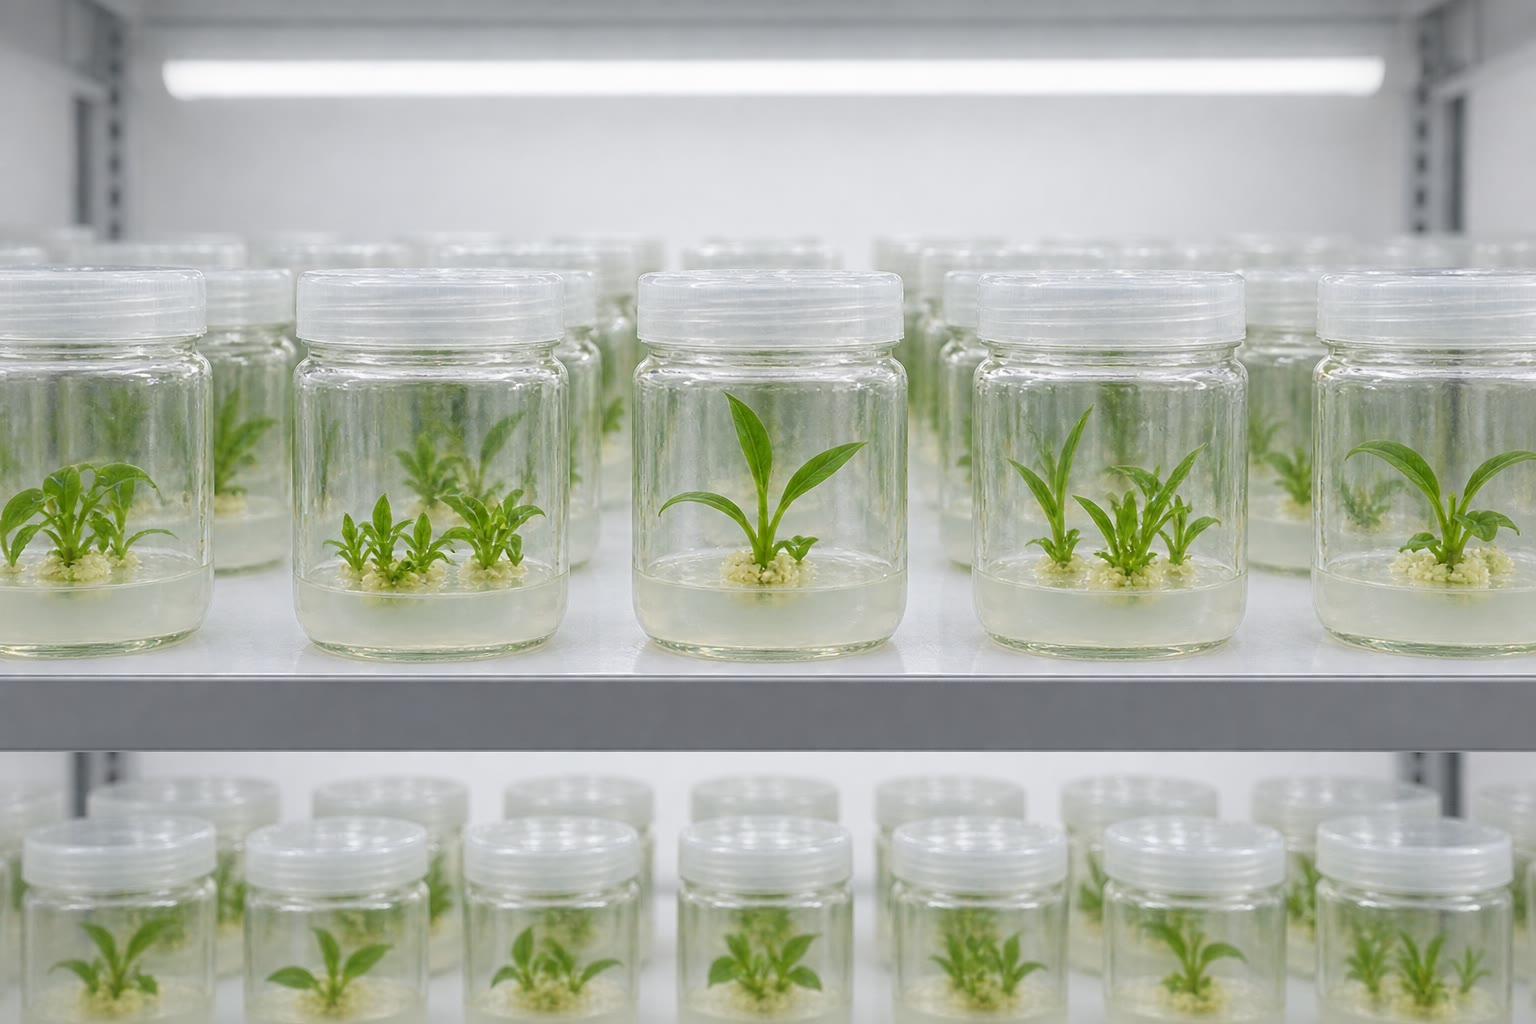
\includegraphics[width=0.6\linewidth]{images/book4/ai/b4-07-tissue-culture.jpg}

{\small Plántulas sobre agar en una cámara de cultivo: cada frasco contiene
un \omterm{def:b2:asexual-reproduction:clone}{clon} de la misma variedad, multiplicado a partir de un solo meristemo.}
\end{omfigure}

\section{El coste del sexo y el coste de prescindir de él}

\begin{theorem}[El doble coste del sexo]\label{thm:b2:asexual-reproduction:twofold}
\index{doble coste del sexo}
En una población en la que cada hembra produce $F$ descendientes, de los
cuales la mitad son machos, una hembra mutante asexual que produce $F$
hijas, todas copias de sí misma, duplica su parte de las hembras de la
generación siguiente. Si el linaje asexual tiene una frecuencia $p$ entre
las hembras, en la generación siguiente
\[
p' = \frac{2p}{1 + p}, \qquad p_t = \frac{2^t p_0}{1 + (2^t - 1)p_0},
\]
de modo que, partiendo de una de cada mil, alcanza la mitad de la
población en diez generaciones y la totalidad poco después. En igualdad
de condiciones, el sexo reduce a la mitad la tasa a la que se multiplica
un linaje --- el precio de producir machos. Como el sexo es, pese a
todo, casi universal, las condiciones no son iguales: los linajes
sexuales deben ganar, en promedio, al menos un factor dos gracias a la
recombinación.
\end{theorem}
\begin{proof}
Las hembras asexuales son $pN$ y dejan $FpN$ hijas; las hembras sexuales
son $(1 - p)N$ y dejan $F(1 - p)N/2$ hijas (la otra mitad son machos, que
no ponen huevos). La parte asexual de las hijas es
$Fp/(Fp + F(1 - p)/2) = 2p/(1 + p)$. Escribiendo $q = p/(1 -
p)$, la recurrencia se convierte en $q' = 2q$, de modo que $q_t = 2^t q_0$;
deshaciendo el cambio de variable se obtiene $p_t$. Imponiendo $p_t = \tfrac12$ se obtiene
$2^t q_0 = 1$, es decir,
$t = \log_2(1/q_0) \approx 10$ para $p_0 = 10^{-3}$.
\end{proof}

\begin{omfigure}
\begin{tikzpicture}
\begin{axis}[
  width=0.76\linewidth, height=5.6cm,
  axis x line=bottom, axis y line=left,
  xmin=0, xmax=20, ymin=0, ymax=1.05,
  xlabel={generaciones}, ylabel={frecuencia del linaje asexual},
  xlabel style={font=\small, at={(axis description cs:0.5,-0.13)}, anchor=north},
  ylabel style={font=\small},
  tick label style={font=\small}, xtick={0,5,10,15,20}, ytick={0,0.5,1},
  legend style={font=\scriptsize, at={(0.5,-0.3)}, anchor=north, draw=none},
  clip=false,
]
\addplot[very thick, omThm, domain=0:20, samples=80] {2^x*0.001/(1+(2^x-1)*0.001)};
\addlegendentry{sin otra diferencia: se impone en 12 generaciones}
\addplot[very thick, omDef, domain=0:20, samples=80] {0.001*(1.3)^x/(1+(1.3^x-1)*0.001)};
\addlegendentry{los asexuales pierden un \qty{35}{\%} de eficacia por parásitos: más lento}
\addplot[very thick, omProp, domain=0:20, samples=80] {0.001*(0.9)^x/(1+(0.9^x-1)*0.001)};
\addlegendentry{los asexuales pierden un \qty{55}{\%}: nunca se extienden}
\end{axis}
\end{tikzpicture}

{\small La doble ventaja en acción. Partiendo de uno por mil, un linaje
asexual sin ninguna otra desventaja se impone en una docena de
generaciones; solo una penalización de eficacia de al menos la mitad
--- por parásitos, \omterm{def:b2:genome-diversification:mutation}{mutaciones} acumuladas o una adaptación más lenta ---
lo frena.}
\end{omfigure}

\begin{proposition}[Para qué sirve el sexo]\label{prop:b2:asexual-reproduction:whysex}
\index{trinquete de Muller}\index{hipótesis de la Reina Roja}
Tres beneficios son lo bastante grandes para importar. \emph{El \omterm{prop:b2:asexual-reproduction:whysex}{trinquete
de Muller}}: en un \omterm{def:b2:asexual-reproduction:clone}{clon}, toda \omterm{def:b2:genome-diversification:mutation}{mutación} perjudicial la heredan todos los
descendientes, y un genoma libre de \omterm{def:b2:genome-diversification:mutation}{mutaciones}, una vez perdido por azar
en una población finita, nunca puede rehacerse; la carga sube como un
trinquete, diente a diente, y las poblaciones asexuales pequeñas
degeneran. La recombinación reconstruye genomas limpios a partir de dos
dañados. \emph{La adaptación}: dos \omterm{def:b2:genome-diversification:mutation}{mutaciones} útiles surgidas en
individuos distintos de un \omterm{def:b2:asexual-reproduction:clone}{clon} compiten y una se pierde; en una
población sexual se combinan (Fisher y Muller, década de 1930), de modo
que las poblaciones sexuales se adaptan más deprisa cuando deben cambiar
muchos genes. \emph{La Reina Roja}: los parásitos se adaptan al \omterm{def:b2:meiosis-heredity:vocabulary}{genotipo}
huésped más común, y un \omterm{def:b2:asexual-reproduction:clone}{clon}, al ser un solo \omterm{def:b2:meiosis-heredity:vocabulary}{genotipo}, es el más común de
todos; los progenitores sexuales hacen de cada descendiente una
cerradura nueva. Los caracoles, los peces y las plantas que tienen a la
vez poblaciones sexuales y clonales muestran que las sexuales predominan
donde abundan los parásitos. Los linajes asexuales que prosperan ---
dientes de león, rotíferos bdeloideos, la mayoría de los \omterm{def:b2:asexual-reproduction:clone}{clones}
cultivados --- son jóvenes, o \omterm{def:b2:genome-diversification:polyploidy}{poliploides} híbridos que llevan su propia
variación, o se sostienen gracias a un cultivador que mata sus parásitos
por ellos.
\end{proposition}

\begin{example}[Monocultivos de un clon]\label{ex:b2:asexual-reproduction:monoculture}
En la década de 1840 la mayor parte de la cosecha de patata de Irlanda
era una sola variedad clonal, la Lumper; el oomiceto \emph{Phytophthora
infestans}, llegado en 1845, se encontró con un país de plantas
genéticamente idénticas y uniformemente sensibles y destruyó la cosecha
tres años seguidos. El plátano de exportación mundial hasta la década de
1950 era un solo \omterm{def:b2:asexual-reproduction:clone}{clon}, Gros Michel, eliminado de las plantaciones de
Centroamérica por un hongo del suelo; su sustituto, Cavendish, es
igualmente un solo \omterm{def:b2:asexual-reproduction:clone}{clon} y lo está perdiendo, plantación tras plantación,
frente a una nueva cepa del mismo hongo, ante la que no tiene variación
alguna que ofrecer. Un \omterm{def:b2:asexual-reproduction:clone}{clon} es el blanco más fácil de la naturaleza, y el
cultivador que planta uno debe aportar la resistencia que la
recombinación habría aportado gratis.
\end{example}

\section{Ejercicios}

\begin{exercise}[$\star$]\label{exo:b2:asexual-reproduction:1}
Defínanse \omterm{def:b2:asexual-reproduction:clone}{clon}, \omterm{def:b2:asexual-reproduction:clone}{geneto} y \omterm{def:b2:asexual-reproduction:clone}{rameto}, y dense tres órganos naturales de
\omterm{def:b2:asexual-reproduction:clone}{multiplicación vegetativa} con una planta para cada uno.
\end{exercise}

\begin{exercise}[$\star$]\label{exo:b2:asexual-reproduction:2}
En un injerto, ¿qué tejidos deben encontrarse para que la unión prospere,
y qué aporta cada uno de los dos al árbol? ¿Por qué un árbol injertado
es una quimera y no un híbrido?
\end{exercise}

\begin{exercise}[$\star$]\label{exo:b2:asexual-reproduction:3}
Distíngase la \omterm{def:b2:asexual-reproduction:apomixis}{apomixis} de la \omterm{def:b2:asexual-reproduction:clone}{multiplicación vegetativa}, y la
\omterm{def:b2:asexual-reproduction:apomixis}{partenogénesis} de ambas. ¿Cuál de las tres conserva la \omterm{def:b2:angiosperm-reproduction:seed}{semilla}?
\end{exercise}

\begin{exercise}[$\star$]\label{exo:b2:asexual-reproduction:4}
Enumérense las etapas de la micropropagación desde el explante hasta la
planta en el campo, indicando las condiciones hormonales de cada una.
\end{exercise}

\begin{exercise}[$\star\star$]\label{exo:b2:asexual-reproduction:5}
Una planta de fresa emite 8 estolones al año, cada uno de los cuales
enraíza 3 plántulas, y cada plántula hace lo mismo al año siguiente.
¿Cuántas plantas hay al cabo de 4 años si no muere ninguna? A razón de
\qty{0.1}{m^2} por planta, ¿qué superficie necesitarían? ¿Qué limita en
realidad el \omterm{def:b2:asexual-reproduction:clone}{clon}?
\end{exercise}

\begin{exercise}[$\star\star$]\label{exo:b2:asexual-reproduction:6}
El \omterm{def:b2:asexual-reproduction:clone}{clon} de álamo temblón Pando tiene \num{47000} troncos sobre
\qty{43}{ha}, y cada tronco vive unos \num{130} años. Si el \omterm{def:b2:asexual-reproduction:clone}{geneto} tiene
\num{14000} años, ¿cuántas generaciones de troncos ha tenido? Calcúlese
su avance radial medio en metros por año, tratándolo como un disco.
\end{exercise}

\begin{exercise}[$\star\star$]\label{exo:b2:asexual-reproduction:7}
Un mutante asexual surge con una frecuencia de $10^{-4}$ en una población
sexual, con la misma fecundidad. Calcúlese su frecuencia al cabo de 5,
10 y 15 generaciones. ¿Cuánto debe reducirse su eficacia para que nunca
se extienda?
\end{exercise}

\begin{exercise}[$\star\star$]\label{exo:b2:asexual-reproduction:8}
Predígase qué hace un callo de tabaco en medios con proporciones auxina :
citoquinina de 10 : 1, 1 : 1 y 1 : 10, y explíquese por qué un esqueje
de tallo se sumerge en auxina y no en citoquinina.
\end{exercise}

\begin{exercise}[$\star\star$]\label{exo:b2:asexual-reproduction:9}
Las patatas se plantan en forma de tubérculos. Un kilogramo plantado
rinde \qty{10}{kg}, y una hectárea necesita \qty{2}{t} de patata de
siembra. Partiendo de \qty{1}{kg} de una variedad nueva, ¿cuántas
temporadas hacen falta para poder plantar una hectárea? ¿Por qué la
\omterm{def:b2:angiosperm-reproduction:seed}{semilla} verdadera permite una multiplicación más rápida y, sin embargo,
no se usa?
\end{exercise}

\begin{exercise}[$\star\star\star$]\label{exo:b2:asexual-reproduction:10}
En una población clonal de $N$ individuos con $U$ \omterm{def:b2:genome-diversification:mutation}{mutaciones} perjudiciales
por genoma y por generación, cada una de las cuales cuesta una fracción
$s$ de la eficacia, la fracción de individuos libres de \omterm{def:b2:genome-diversification:mutation}{mutaciones} en el
equilibrio es
$e^{-U/s}$ (se deduce en el \cref{ch:b2:population-genetics}). Con $U =
0.1$ y $s = 0.02$, calcúlese el número de individuos libres de \omterm{def:b2:genome-diversification:mutation}{mutaciones}
para $N = 10^{5}$ y $N = 10^{3}$, y explíquese, con el \omterm{prop:b2:asexual-reproduction:whysex}{trinquete de
Muller}, por qué la población pequeña está condenada y la grande no ---
todavía.
\end{exercise}

\begin{exercise}[$\star\star\star$]\label{exo:b2:asexual-reproduction:11}
Una cepa de patógeno que vence la resistencia de un \omterm{def:b2:meiosis-heredity:vocabulary}{genotipo} dado surge
una vez. Compárese su destino en un campo de un solo \omterm{def:b2:asexual-reproduction:clone}{clon} y en una
población sexual en la que los genes de resistencia segregan en diez
loci, cada uno con dos \omterm{def:b2:meiosis-heredity:vocabulary}{alelos} de igual frecuencia, y explíquese en estos
términos la gran hambruna irlandesa de la patata.
\end{exercise}

\begin{exercise}[$\star\star\star$]\label{exo:b2:asexual-reproduction:12}
``El sexo cuesta un factor dos y está en todas partes; la asexualidad es
barata y rara.'' Discútanse las tres explicaciones del capítulo, y
dígase qué implican para cada una los rotíferos bdeloideos, asexuales
desde hace cuarenta millones de años.
\end{exercise}

\section{Problema: un fresal y un clon antiguo}

\begin{problem}[{Problema de fin de semana --- la aritmética de un clon,
desde un campo de fresas que se llena por estolones y un laboratorio que
multiplica un meristemo hasta la invasión de una población sexual por un
apomíctico y la degeneración genética de un geneto antiguo, hasta llegar
al tiempo necesario para llenar el campo, las plántulas que da un
meristemo y el equilibrio entre apomícticos y sexuales}]
\label{pb:b2:asexual-reproduction:1}
Un agricultor planta \num{100} plantas de fresa en un campo de
\qty{1}{ha} que admite \num{4} plantas por metro cuadrado. Cada planta
emite \num{6} estolones al año, cada uno de los cuales enraíza \num{2}
hijas, y todas las plantas sobreviven. Un laboratorio multiplica la misma
variedad por cultivo de tejidos: cada subcultivo, cada \num{4} semanas,
multiplica los brotes por \num{5}; el \qty{80}{\%} de las plántulas
sobrevive a la aclimatación. Los esquejes ordinarios de la variedad
están infectados por virus en un \qty{90}{\%}; los ápices meristemáticos
de \qty{0.3}{mm} llevan el virus con probabilidad $0.02$. Genoma del
álamo temblón: \qty{4.8e8}{} pares de bases; \omterm{thm:b2:genome-diversification:rate}{tasa de mutación} somática
de \qty{1e-9}{} por par de bases y por división celular; \num{20}
divisiones de las células del meristemo al año en un brote en
crecimiento.

\medskip
\noindent\textbf{Parte I --- Llenar el campo.}
\begin{enumerate}
  \item ¿Cuántas plantas admite el campo?
  \item ¿Por qué factor se multiplica cada año el número de plantas?
  \item Calcúlese el número de plantas al cabo de 1, 2 y 3 años.
  \item Resuélvase $N(t) = 100\times 13^{t}$ para hallar el momento en
        que el campo está lleno.
  \item Una vez lleno, solo las plantas del borde de una mancha encuentran
        sitio. Si una mancha avanza \qty{0.5}{m} al año, ¿cuántos años
        tardaría una sola planta en cubrir el campo solo por avance?
  \item Explíquese por qué el agricultor planta \num{100} plantas
        repartidas por el campo en lugar de una.
\end{enumerate}

\medskip
\noindent\textbf{Parte II --- El laboratorio.}
\begin{enumerate}[resume]
  \item ¿Cuántos subcultivos hacen falta para pasar de un meristemo a al
        menos $10^{6}$ brotes? ¿Cuántas semanas?
  \item ¿Cuántas plantas sobreviven a la aclimatación?
  \item ¿Cuál es la probabilidad de que una línea derivada de un
        meristemo esté libre de virus? ¿Y de que lo estén las \num{10}
        líneas iniciadas a partir de una misma planta?
  \item El laboratorio inicia \num{10} líneas y descarta las infectadas
        tras un análisis. ¿Número esperado de líneas limpias? Compárese
        con los esquejes.
  \item Explíquese por qué el ápice del meristemo escapa al virus.
  \item El campo podría plantarse con la producción del laboratorio el
        primer año en lugar de llenarse por estolones en tres. Dense una
        ventaja y un riesgo de cada vía.
\end{enumerate}

\medskip
\noindent\textbf{Parte III --- Un apomíctico invade.}
Una población de dientes de león es sexual; un mutante apomíctico (que se
clona por \omterm{def:b2:angiosperm-reproduction:seed}{semillas}) aparece con una frecuencia $p_0 = 10^{-3}$ y la misma
producción de \omterm{def:b2:angiosperm-reproduction:seed}{semillas} por planta. La mitad del esfuerzo reproductivo de
las plantas sexuales se destina al \omterm{def:b2:plant-life-cycles:heterospory}{polen}.
\begin{enumerate}[resume]
  \item Justifíquese la recurrencia $p' = 2p/(1 + p)$ para la frecuencia
        del apomíctico entre los progenitores de \omterm{def:b2:angiosperm-reproduction:seed}{semillas}.
  \item Calcúlese $p$ al cabo de 5 y de 10 generaciones, y la generación
        en la que supera la mitad.
  \item Una roya se especializa en el \omterm{def:b2:meiosis-heredity:vocabulary}{genotipo} más común: la producción de
        \omterm{def:b2:angiosperm-reproduction:seed}{semillas} del apomíctico se reduce en un factor $(1 - cp)$, con
        $c = 0.8$. Escríbase la nueva recurrencia.
  \item Hállese la frecuencia de equilibrio $p^*$ y compruébese su
        estabilidad a partir del signo de $p' - p$ a ambos lados.
  \item ¿Para qué valores de $c$ se impone por completo el apomíctico?
  \item Calcúlese el equilibrio para $c = 0.6$. Interprétese: ¿qué debe
        hacer un parásito para proteger el sexo?
  \item El apomíctico es triploide. ¿Por qué no puede volver al sexo, y
        por qué importa esto a largo plazo?
\end{enumerate}

\medskip
\noindent\textbf{Parte IV --- El \omterm{def:b2:asexual-reproduction:clone}{clon} antiguo.}
\begin{enumerate}[resume]
  \item Calcúlese el número de \omterm{def:b2:genome-diversification:mutation}{mutaciones} somáticas por división celular
        en el álamo temblón.
  \item Dos troncos del \omterm{def:b2:asexual-reproduction:clone}{clon} Pando están separados por \num{14000} años
        de crecimiento a cada lado de su antepasado común. ¿Cuántas
        divisiones celulares los separan, y cuántas \omterm{def:b2:genome-diversification:mutation}{mutaciones} distinguen
        sus genomas?
  \item ¿Qué fracción del genoma representa eso? Si el \qty{2}{\%} del
        genoma es codificante, ¿cuántas diferencias codificantes hay?
  \item Un \omterm{def:b2:asexual-reproduction:clone}{clon} no tiene \omterm{def:b2:meiosis-heredity:meiosis}{meiosis} ni selección a escala del organismo que
        elimine estas \omterm{def:b2:genome-diversification:mutation}{mutaciones}. ¿Qué las elimina, y por qué ese filtro
        es más débil que en un linaje sexual?
  \item ¿Es Pando ``genéticamente uniforme''? Discútase en dos frases.
  \item Enúnciese el resultado: el tiempo necesario para llenar el campo
        por estolones, las plántulas que da un meristemo en un año y la
        frecuencia de equilibrio del apomíctico para $c = 0.8$.
\end{enumerate}
\end{problem}
